\documentclass{beamer}
\usepackage[latin1]{inputenc}
\usepackage{xcolor}
\usepackage{hyperref}
\usepackage{minted}
\usepackage{graphicx}
\usepackage{tikz}
\usetikzlibrary{fadings,tikzmark,calc,positioning,decorations.pathreplacing}
\usepackage{bbding} % For \HandRight
\usepackage{fancyvrb} % For \UseVerb \SaveVerb

\usetheme{Madrid}
\usecolortheme{default}

% Command that embeds a hand pointing to the right in a href label
\newcommand{\hrefhand}[2]{\raisebox{-0.4ex}{\HandRight}\,\href{#1}{#2}}

\title{COMP3320 Introduction to OpenGL}
\author{Alex Biddulph}
\institute{
    The University of Newcastle, Australia
    \and
    Based on the work provided at \url{www.learnopengl.com}
}
\date{Semester 2, 2021}

\begin{document}

\begin{frame}
    \titlepage
\end{frame}

\begin{frame}[fragile]{Vertex Attributes}
    \SaveVerb{glVertexAttribPointer}|glVertexAttribPointer|
    \begin{itemize}
        \item Allows us to specify auxiliary data for each vertex
        \item Specify offset and stride using \hrefhand{https://www.khronos.org/registry/OpenGL-Refpages/gl4/html/glVertexAttribPointer.xhtml}{\color{blue}\UseVerb{glVertexAttribPointer}}
        \item An example specifying vertex colour information
              \footnotesize{
                  \begin{minted}{c++}
    float vertices[] = {
         0.5f, -0.5f, 0.0f,  1.0f, 0.0f, 0.0f,
        -0.5f, -0.5f, 0.0f,  0.0f, 1.0f, 0.0f,
         0.0f,  0.5f, 0.0f,  0.0f, 0.0f, 1.0f };
\end{minted}
              }
    \end{itemize}

    \begin{figure}
        \centering
        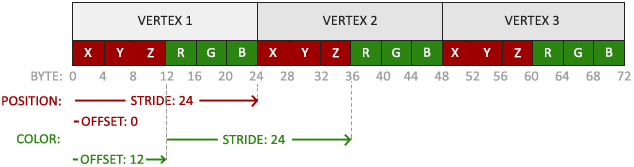
\includegraphics[width=0.90\linewidth,keepaspectratio=true]{images/vertex_attribute_pointer_interleaved.png}
        \caption{\footnotesize{Image sourced from \url{learnopengl.com/Getting-started/Shaders}}}
    \end{figure}

    \begin{tikzpicture}[remember picture, overlay]
        \node[rectangle,minimum width=3.25cm,minimum height=1.25cm,draw=red,ultra thick] at (3.65cm, 5.45cm) (P) {};
        \node[rectangle,minimum width=3.20cm,minimum height=1.25cm,draw=green,ultra thick] at (7.00cm, 5.45cm) (C) {};
        \draw[ultra thick,red,->] (P.south west) -- (2.50cm, 3.90cm);
        \draw[ultra thick,green,->] (C.south west) -- (4.50cm, 3.90cm);
    \end{tikzpicture}
\end{frame}

\begin{frame}[fragile]{Vertex Attributes}
    Result should look like this
    \begin{center}
        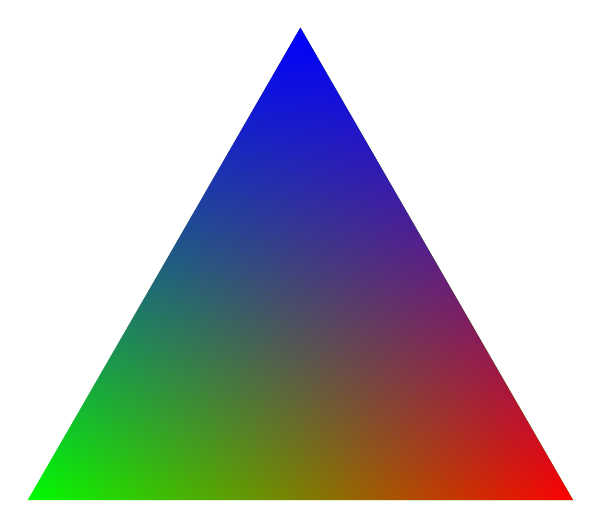
\begin{tikzpicture}
            \fill[green] (90:4) -- (210:4) -- (-30:4) -- cycle;
            \fill[red,path fading=west] (90:4) -- (210:4) -- (-30:4) -- cycle;
            \fill[blue,path fading=south] (90:4) -- (210:4) -- (-30:4) -- cycle;
        \end{tikzpicture}
    \end{center}
\end{frame}

\begin{frame}[fragile]{Textures}
    \begin{itemize}
        \item Rather than using colours to add detail to an object, use an image
        \item Easier to add a lot of detail to an object
        \item To apply a texture we just need to assign texture coordinates to each vertex
              \footnotesize{
                  \begin{minted}{c++}
float vertices[] = {
     0.5f, -0.5f, 0.0f,  1.0f, 0.0f, 0.0f, 1.0f, 0.0f,
    -0.5f, -0.5f, 0.0f,  0.0f, 1.0f, 0.0f, 0.0f, 0.0f,
     0.0f,  0.5f, 0.0f,  0.0f, 0.0f, 1.0f, 0.5f, 1.0f };
\end{minted}
              }
    \end{itemize}

    \begin{figure}
        \centering
        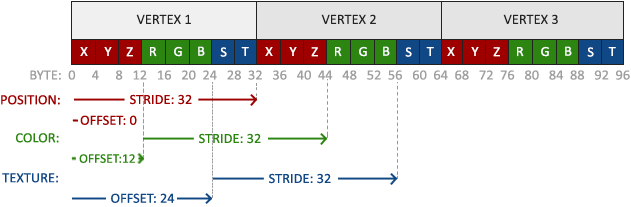
\includegraphics[width=0.90\linewidth,keepaspectratio=true]{images/vertex_attribute_pointer_interleaved_textures.png}
        \caption{\footnotesize{Image sourced from \url{learnopengl.com/Getting-started/Textures}}}
    \end{figure}

    \begin{tikzpicture}[remember picture, overlay]
        \node[rectangle,minimum width=3.25cm,minimum height=1.25cm,draw=red,ultra thick] at (3.00cm, 5.85cm) {};
        \node[rectangle,minimum width=3.00cm,minimum height=1.25cm,draw=green,ultra thick] at (6.25cm, 5.85cm) {};
        \node[rectangle,minimum width=1.90cm,minimum height=1.25cm,draw=blue,ultra thick] at (8.80cm, 5.85cm) {};
    \end{tikzpicture}
\end{frame}

\begin{frame}[fragile]{Texture Wrapping}
    \SaveVerb{glTexParameteri}|glTexParameteri|
    \SaveVerb{glTexParameterfv}|glTexParameterfv|
    \begin{itemize}
        \item Texture coordinates range from $\left(0, 0\right) \to \left(1, 1\right)$
        \item What should happen if coordinates outside this range are specified?
    \end{itemize}

    \begin{examples}
        Specify texture wrapping behaviour using \hrefhand{https://www.khronos.org/registry/OpenGL-Refpages/gl4/html/glTexParameter.xhtml}{\color{blue}\UseVerb{glTexParameteri}}
    \end{examples}
    \begin{examples}
        Specify texture border colour using \hrefhand{https://www.khronos.org/registry/OpenGL-Refpages/gl4/html/glTexParameter.xhtml}{\color{blue}\UseVerb{glTexParameterfv}}
    \end{examples}

    \begin{figure}
        \centering
        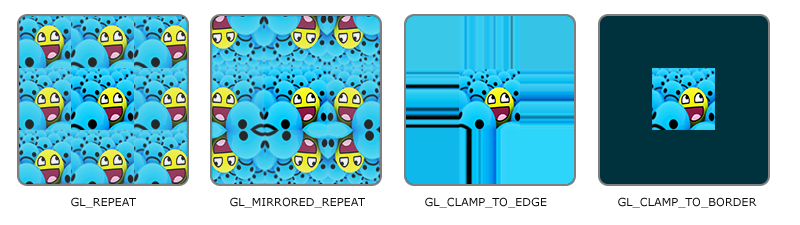
\includegraphics[width=0.90\linewidth,keepaspectratio=true]{images/texture_wrapping.png}
        \caption{\footnotesize{Image sourced from \url{learnopengl.com/Getting-started/Textures}}}
    \end{figure}
\end{frame}

\begin{frame}[fragile]{Texture Filtering}
    \begin{itemize}
        \item Floating-point coordinates are mapped to integer coordinates
        \item What should happen if texture coordinates have a fractional component? For example, $\left(0.75, 0.0\right) \rightarrow \left(480.3, 300\right)$
        \item Behaviour can be specified for both minifying and magnifying operations
    \end{itemize}

    \SaveVerb{glTexParameteri}|glTexParameteri|
    \begin{examples}
        Specify texture filtering behaviour using \hrefhand{https://www.khronos.org/registry/OpenGL-Refpages/gl4/html/glTexParameter.xhtml}{\color{blue}\UseVerb{glTexParameteri}}
    \end{examples}

    \begin{figure}
        \centering
        
\includegraphics[height=0.25\textwidth,keepaspectratio=true]{images/texture_filtering.png}
        \caption{\footnotesize{Image sourced from \url{learnopengl.com/Getting-started/Textures}}}
    \end{figure}
\end{frame}

\begin{frame}[fragile]{MipMaps}
    \begin{itemize}
        \item No need to use a high resolution image to texture an object a long distance away
        \item Can also result in undesirable artifacts on small objects
        \item The solution?
              \begin{itemize}
                  \item Create multiple scaled down versions of the high resolution image
                  \item Select a different scaled down texture based on the distance from the camera
              \end{itemize}
        \item Behaviour can be specified for both minifying and magnifying operations
    \end{itemize}

    \SaveVerb{glGenerateMipmaps}|glGenerateMipmaps|
    \begin{examples}
        OpenGL will generate mipmaps for you. Use \hrefhand{https://www.khronos.org/registry/OpenGL-Refpages/gl4/html/glGenerateMipmap.xhtml}{\color{blue}\UseVerb{glGenerateMipmaps}}
    \end{examples}
\end{frame}

\begin{frame}[fragile]{MipMaps}
    \begin{figure}
        \centering
        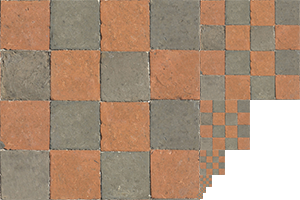
\includegraphics[height=0.75\textheight,keepaspectratio=true]{images/mipmaps.png}
        \caption{\footnotesize{Image sourced from \url{learnopengl.com/Getting-started/Textures}}}
    \end{figure}
\end{frame}

\begin{frame}[fragile]{Loading Textures}
    \begin{itemize}
        \item A number of C/C++ libraries available for loading images
        \item SOIL is a common library specifically targetting OpenGL
    \end{itemize}

    \SaveVerb{glGenTextures}|glGenTextures|
    \SaveVerb{glBindTexture}|glBindTexture|
    \SaveVerb{glTexImage2D}|glTexImage2D|
    \begin{examples}
        Generate a OpenGL texture object using \hrefhand{https://www.khronos.org/registry/OpenGL-Refpages/gl4/html/glGenTextures.xhtml}{\color{blue}\UseVerb{glGenTextures}}
    \end{examples}
    \begin{examples}
        Bind a texture object and make it the active texture using \hrefhand{https://www.khronos.org/registry/OpenGL-Refpages/gl4/html/glBindTexture.xhtml}{\color{blue}\UseVerb{glBindTexture}}
    \end{examples}
    \begin{examples}
        Use \hrefhand{https://www.khronos.org/registry/OpenGL-Refpages/gl4/html/glTexImage2D.xhtml}{\color{blue}\UseVerb{glTexImage2D}} to attach the raw texture data to the currently active texture unit. After this you can delete any pointers to your raw texture data
    \end{examples}
\end{frame}

\begin{frame}[fragile]{Texture Units}
    \begin{itemize}
        \item Multiple textures can be used in a single program
        \item Each texture needs to be attached to a different texture unit
    \end{itemize}

    \SaveVerb{glGetIntegerv}|glGetIntegerv|
    \SaveVerb{glActiveTexture}|glActiveTexture|
    \begin{examples}
        Query {\color{blue}\verb"GL_MAX_TEXTURE_IMAGE_UNITS"} using \hrefhand{https://www.khronos.org/registry/OpenGL-Refpages/gl4/html/glGet.xhtml}{\color{blue}\UseVerb{glGetIntegerv}} to find the maximum available on your hardware
    \end{examples}
    \begin{examples}
        Use \hrefhand{https://www.khronos.org/registry/OpenGL-Refpages/gl4/html/glActiveTexture.xhtml}{\color{blue}\UseVerb{glActiveTexture}} to select currently active texture unit
    \end{examples}
\end{frame}

\begin{frame}[fragile]{Textures}
    Result should look like this

    \begin{figure}
        \centering
        \begin{tikzpicture}[baseline={([yshift=-1em] current bounding box.north)}]
            % Grid lines
            \draw[step=0.5,lightgray,thin] (-1.5, -1.5) grid (1.5, 1.5);

            % Window edges
            \draw[thick] (-1.5, -1.5) -- (-1.5, 1.5) -- (1.5, 1.5) -- (1.5, -1.5) -- cycle;

            % Triangle
            \def\triangle{(-1.5, -1.5) -- (0.0, 1.5) -- (1.5, -1.5) -- cycle}
            \begin{scope}
                \clip \triangle;
                \node {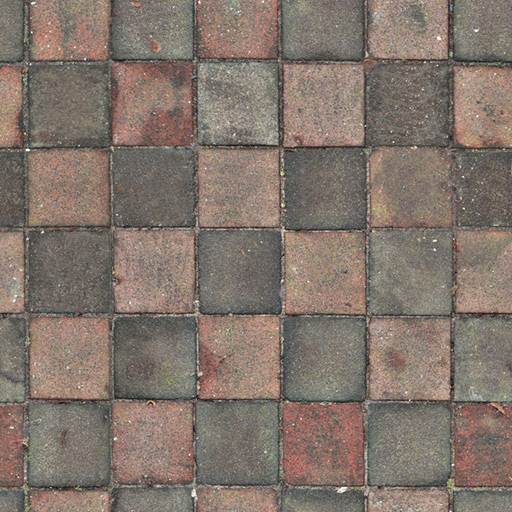
\includegraphics[width=0.3\linewidth]{images/wall.jpg}};
            \end{scope}
            \draw[black, thick] \triangle;

            % Coordinates
            \draw (-1.5, -1.5) node[below left]{$\left(0, 0\right)$};
            \draw ( 1.5,  1.5) node[above right]{$\left(1, 1\right)$};
            \draw (-1.5,  1.5) node[above left]{$\left(0, 1\right)$};
            \draw ( 1.5, -1.5) node[below right]{$\left(1, 0\right)$};
        \end{tikzpicture}
        \caption{\footnotesize{Brick wall image sourced from \url{learnopengl.com/Getting-started/Textures}}}
    \end{figure}
\end{frame}

\end{document}
